\documentclass[aspectratio=169]{beamer}

% Theme and Color
\usetheme{metropolis}
\usecolortheme{seahorse}

% Packages
\usepackage{graphicx}
\usepackage{booktabs}
\usepackage{hyperref}
\usepackage{tikz}
\usepackage{pgfplots}
\pgfplotsset{compat=1.18}
\usetikzlibrary{shapes.geometric, arrows.meta, positioning, fit, backgrounds}

% Title Information
\title{\textbf{8 Ball}}
\subtitle{Real-Time NBA Analytics Platform}
\author{Ben Aoki-Sherwood \and Arjun Ashok Rao}
\institute{CSCI 5253: Datacenter Scale Computing \\ University of Colorado Boulder}
\date{December 2025}

% Remove navigation symbols
\setbeamertemplate{navigation symbols}{}

% Footer with slide numbers
\setbeamertemplate{footline}[frame number]

\begin{document}

% =============================================================================
% TITLE SLIDE
% =============================================================================
\begin{frame}
\titlepage
\end{frame}

% =============================================================================
% PROBLEM STATEMENT
% =============================================================================
\begin{frame}{What is \textbf{8 Ball}?}

\begin{itemize}
    \item Follow your favorite teams and players: real-time NBA game stats and analytics
    \item See who's on top: track standings and leaderboards over the course of the season
    \item Scale to hundreds of concurrent users
\end{itemize}

\end{frame}

\begin{frame}{Tech Stack}
\begin{itemize}
    \item \textbf{Backend:} Python, FastAPI, PostgreSQL, Redis
    \item \textbf{Frontend:} Next.js, TypeScript, Material-UI
    \item \textbf{Cloud:} GCP Cloud Run, Cloud SQL, Memorystore
    \item \textbf{IaC:} Terraform, Docker
\end{itemize}
    
\end{frame}

% =============================================================================
% SYSTEM ARCHITECTURE
% =============================================================================
\begin{frame}{System Architecture}

\begin{figure}
\centering
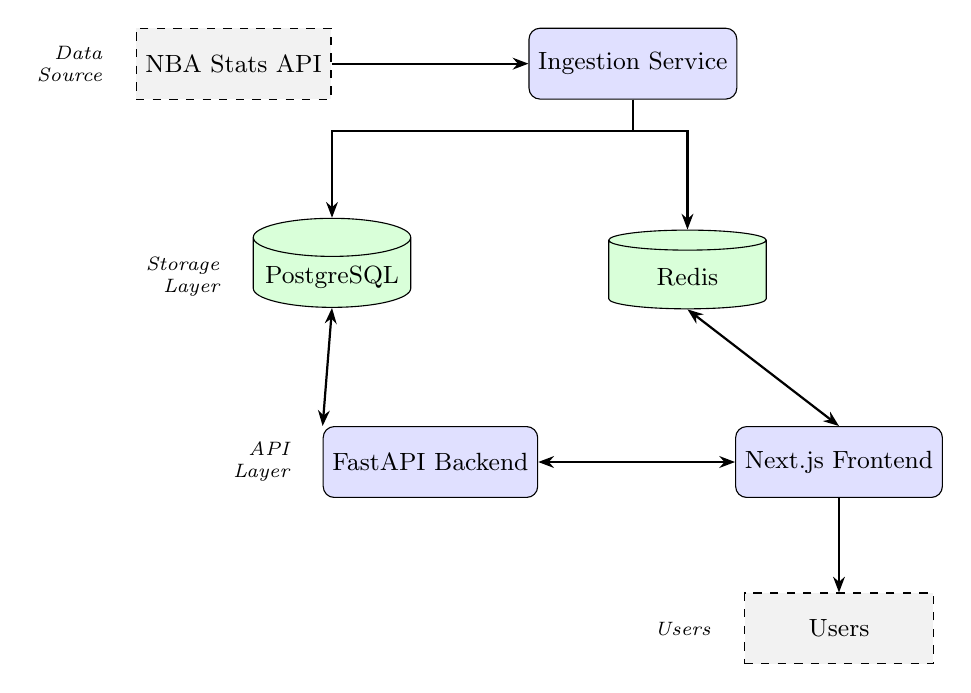
\begin{tikzpicture}[
    node distance=1.2cm,
    component/.style={rectangle, draw, rounded corners, minimum width=2.4cm, minimum height=0.9cm, align=center, fill=blue!12, font=\small},
    database/.style={cylinder, draw, shape border rotate=90, aspect=0.25, minimum height=1cm, minimum width=2cm, fill=green!15, font=\small},
    external/.style={rectangle, draw, dashed, minimum width=2.4cm, minimum height=0.9cm, align=center, fill=gray!10, font=\small},
    arrow/.style={-{Stealth[length=2mm]}, thick},
    biarrow/.style={{Stealth[length=2mm]}-{Stealth[length=2mm]}, thick}
]

% Row 1: Data ingestion
\node[external] (nba) {NBA Stats API};
\node[component, right=2.5cm of nba] (ingestion) {Ingestion Service};

% Row 2: Storage layer
\node[database, below=1.5cm of nba, xshift=1.25cm] (postgres) {PostgreSQL};
\node[database, right=2.5cm of postgres] (redis) {Redis};

% Row 3: API and Frontend
\node[component, below=1.5cm of postgres, xshift=1.25cm] (api) {FastAPI Backend};
\node[component, right=2.5cm of api] (frontend) {Next.js Frontend};

% Users
\node[external, below=1.2cm of frontend] (users) {Users};

% Arrows - Ingestion flow
\draw[arrow] (nba) -- (ingestion);
\draw[arrow] (ingestion.south) -- ++(0,-0.4) -| (postgres.north);
\draw[arrow] (ingestion.south) -- ++(0,-0.4) -| (redis.north);

% Arrows - API reads from storage
\draw[biarrow] (postgres.south) -- (api.north west);
\draw[biarrow] (redis.south) -- (frontend.north);

% Arrows - Frontend and users
\draw[biarrow] (api) -- (frontend);
\draw[arrow] (frontend) -- (users);

% Layer labels
\node[left=0.3cm of nba, font=\scriptsize\itshape, align=right] {Data\\Source};
\node[left=0.3cm of postgres, font=\scriptsize\itshape, align=right] {Storage\\Layer};
\node[left=0.3cm of api, font=\scriptsize\itshape, align=right] {API\\Layer};
\node[left=0.3cm of users, font=\scriptsize\itshape, align=right] {Users};

\end{tikzpicture}
\end{figure}

\begin{itemize}
    \item \textbf{Ingestion:} NBA API $\rightarrow$ PostgreSQL + Redis (0.6s rate limit)
    \item \textbf{API:} FastAPI cache-first queries (85\%+ hit rate, <150ms avg)
    \item \textbf{Frontend:} Next.js client-side rendering with auto-refresh
    \item \textbf{Cloud:} Auto-scaling Cloud Run (0-10 API, 0-5 frontend instances)
\end{itemize}

\end{frame}

% =============================================================================
% KEY FEATURES
% =============================================================================
\begin{frame}{Key Features}

\begin{columns}[T]
\begin{column}{0.5\textwidth}
\textbf{Data \& Analytics:}
\begin{itemize}
    \item 2 seasons of historical data (2024-2026)
    \item Live game updates every 15-30 seconds
    \item Statistical leaders (PTS, REB, AST, STL, BLK)
    \item Conference standings with streaks
    \item Team performance analysis
\end{itemize}
\end{column}

\begin{column}{0.5\textwidth}
\textbf{Visualizations:}
\begin{itemize}
    \item \textbf{3D Shot Charts:} Plotly.js with parabolic arcs
    \item \textbf{2D Heatmaps:} Recharts with full court rendering
    \item \textbf{Play-by-Play:} Real-time event feed with icons
    \item \textbf{Box Scores:} Quarterly scoring tables
    \item \textbf{Team Trends:} Point differential over season
\end{itemize}
\end{column}
\end{columns}

\end{frame}

% =============================================================================
% PERFORMANCE METRICS
% =============================================================================
\begin{frame}{Scalability \& Debugging}

\begin{columns}[T]
\begin{column}{0.55\textwidth}
\textbf{Debugging and testing:}

\begin{itemize}
    \item FastAPI autodocs
    \item Browser devtools console; tested on multiple browsers and platforms
    \item \texttt{pytest} unit testing framework
    \item Manual end-to-end testing for a week's worth of games
    \item pydantic type checking for debugging
\end{itemize}
\end{column}

\begin{column}{0.45\textwidth}
\textbf{Bottlenecks:}
\begin{enumerate}
    \item NBA API rate limit (0.6s/req)
    \item Statistical leader queries (200ms)
    \item Plotly.js bundle size (3MB)
\end{enumerate}

\vspace{0.5em}
\textbf{Solutions:}
\begin{itemize}
    \item Redis caching (1hr TTL for leaders)
    \item Lazy loading for 3D charts
    \item Incremental ingestion mode
    \item Client-side rendering
\end{itemize}
\end{column}
\end{columns}

\end{frame}

\begin{frame}[standout]
    Demo
\end{frame}

% =============================================================================
% LESSONS LEARNED
% =============================================================================
% \begin{frame}{Lessons Learned \& Future Work}

% \begin{columns}[T]
% \begin{column}{0.5\textwidth}
% \textbf{Technical Challenges:}
% \begin{itemize}
%     \item NBA API inconsistencies (null fields in live data)
%     \item Time zone conversions (UTC $\rightarrow$ Eastern)
%     \item Redis schema migrations during development
%     \item CORS configuration for frontend-backend
% \end{itemize}

% \vspace{0.5em}
% \textbf{Best Practices:}
% \begin{itemize}
%     \item Pydantic type safety caught 15+ bugs
%     \item Docker Compose for one-command dev setup
%     \item Terraform for reproducible infrastructure
% \end{itemize}
% \end{column}

% \begin{column}{0.5\textwidth}
% \textbf{Future Enhancements:}
% \begin{enumerate}
%     \item \textbf{ML Predictions:} LSTM models for game outcomes
%     \item \textbf{Horizontal Scaling:} Multi-instance API + read replicas
%     \item \textbf{Monitoring:} Prometheus + Grafana dashboards
%     \item \textbf{Real-time Alerts:} WebSocket push for live scores
%     \item \textbf{Player Comparisons:} Side-by-side stat analysis
% \end{enumerate}
% \end{column}
% \end{columns}

% \vspace{1em}
% \begin{center}
% \Large{\textbf{Thank You! Questions?}}
% \end{center}

% \end{frame}

\end{document}
